\documentclass{article}
\usepackage{fullpage}
\usepackage[per-mode=symbol]{siunitx}
\usepackage{amsmath}
\usepackage{empheq}
\usepackage{tikz}
\usepackage{mathtools}
\usetikzlibrary{shapes,arrows,positioning}

\tikzstyle{block} = [draw, fill=white, rectangle, 
minimum height=3em, minimum width=6em]
\tikzstyle{sum} = [draw, fill=white, circle, node contents=$\sum$]
\tikzstyle{gain} = [draw, fill=white, circle]
\tikzstyle{suminplus} = [very near end,node contents=$+$]
\tikzstyle{suminminus} = [very near end,node contents=$-$]
\tikzstyle{input} = []
\tikzstyle{output} = []

\DeclarePairedDelimiter{\norm}{\lVert}{\rVert}
\DeclareMathOperator{\tanc}{tanc}


\renewcommand{\vec}{\boldsymbol} % Use bold vectors instead of arrows
\newcommand{\mat}{\vec}
\newcommand{\evec}[1]{\vec{\hat{#1}}}
\newcommand{\uvec}[1]{\vec{\hat{#1}}}
\newcommand{\dvec}[1]{\vec{\dot{#1}}}
\newcommand{\tvec}[1]{\vec{\tilde{#1}}}
\newcommand{\etvec}[1]{\vec{\hat{\tilde{#1}}}}
\newcommand{\bmat}[1]{\begin{bmatrix} #1 \end{bmatrix}}

\title{Target Altitude Control for Deployable Air Brake System (DABS)}
\date{Spring 2020}
\author{Patrick Love}

\begin{document}
	
	\maketitle
	
	\section{Apogee Prediction}
	
	For the initial semester objective, the apogee prediction will use a relatively simple model under the assumption of perfectly vertical flight and simple square-law drag.  This reduces the problem to 1D and as we will see permits an analytic prediction of the maximum altitude given the current altitude and velocity.  In this analysis we will denote the altitude by $z$.  We begin as always by defining the forces acting on our body, in this case drag and gravity.
	
	\begin{equation}
		F = -\frac{1}{2}C_d\rho A\dot{z}^2-mg
	\end{equation}
	
	Instead of the usual technique using $F=\dot{p}=m\ddot{z}$ we instead employ the less common $F=\frac{dE}{dz}=m\frac{d\epsilon}{dz}$ noting that $\epsilon=\frac{1}{2}\dot{z}^2$ allows us to also express the drag force as directly proportional to (specific) energy\footnote{There is no potential energy term included in the energy since gravity is already being modeled as a force instead}.  This reduces the differential equation to first-order \textit{and} the independent variable is now $z$, which is what we are ultimately interested in.  With these substitutions and dividing through by the mass the equation of motion becomes:
	
	\begin{equation}
		\frac{d\epsilon}{dz} = -\frac{C_d\rho A}{m}\epsilon-g 
	\end{equation}
	
	Here we will define a sort of 'drag constant' $K = \frac{C_d\rho A}{m} $ with units [\si{\per\meter}] which simplifies the equation to:
	
	\begin{equation}
	\label{eqn:vertde}
	\frac{d\epsilon}{dz} = -K\epsilon-g 
	\end{equation}
	
	This could in principle be solved as is using the general first order ODE solution, but it will prove easier to incorporate the initial values and solve for the quantity of interest (apogee) if we make the equation separable using the change of variable $\epsilon_* = \epsilon+\frac{g}{K}$.  I have yet to come of with a good intuitive interpretation of $\epsilon_*$, but I will call it the augmented specific energy.  Using this variable the equation is simplified further:
	
	\begin{equation}
	\frac{d\epsilon_*}{dz} = -K\epsilon_*
	\end{equation}
	
	While the exponential solution for $\epsilon_*(x)$ is obvious, we are actually going to carry through the integration process as it will very naturally allow us to enforce the desired boundary conditions.  Separating and integrating yields:
	
	\begin{equation}
	-\frac{1}{K}\int\epsilon_*^{-1}d\epsilon_* = \int dz
	\end{equation}
	
	But what should be the bounds of the integrals?  Well conveniently the lower (initial) bounds are derived exactly from the initial altitude and velocity given.  However we can also set the upper bound to represent apogee \textit{right now} since we already know $\dot{z}=\epsilon=0$ at apogee, and the other limit is just the final apogee altitude $z_A$ we want to solve for.  Integrating over these bounds yields:
	 
	\begin{equation}
	-\frac{1}{K}\left[\ln\left(\epsilon_*\right)\right]_{\epsilon_0+\frac{g}{K}}^{\frac{g}{K}} = z_A - z_0
	\end{equation}
	
	Manipulating this result gets us to our final expression for $z_A$:
	
	\begin{equation}
	z_A = z_0 + \frac{1}{K}\left[\ln\left(\epsilon_0+\frac{g}{K}\right)-\ln\frac{g}{K}\right]
	\end{equation}
	
	\begin{empheq}[box=\fbox]{equation}
	\label{eqn:kapogee} z_A = z_0 + \frac{1}{K}\ln\left(1 + \frac{K}{g}\epsilon_0\right) = z_0 + \frac{1}{K}\ln\left(1 + \frac{K}{2g}v_0^2\right)
	\end{empheq}
	
	We can check that this result makes sense by examining the limit as $K$ (the drag) goes to zero as below:
	
	\begin{align}
		\Delta z &= \lim\limits_{K\rightarrow0} \frac{1}{K}\ln\left(1 + \frac{K}{g}\epsilon_0\right) \\
		&=\lim\limits_{K\rightarrow0}\ln\left(1 + \frac{K}{g}\epsilon_0\right)^\frac{1}{K} \\
		&=\lim\limits_{n\rightarrow\infty}\ln\left(1+\frac{1}{n}\right)^{n\cdot \frac{\epsilon_0}{g}}\qquad n=\frac{g}{K\epsilon_0} \\
		&=\ln e^{\frac{\epsilon_0}{g}} = \frac{\epsilon_0}{g}
	\end{align}
	
	This is exactly the effect of pure gravitational potential energy $g\Delta z = \epsilon_0\ \rightarrow\ mg\Delta z = E_0$ as we would expect without the presence of air resistance.  We can make the result more intuitive noting that the inverse solution for $\epsilon_0$ of $z_A$ is primarily an exponential $e^{K\Delta z}$.  When dealing with these sorts of exponentials, it can often be more intuitive to consider a sort of 'characterstic interval' (like the time constant of an RC circuit) rather than a decay rate.  Indeed let us define $L_d = \frac{1}{K} = \frac{m}{C_p\rho A}$ as the characteristic drag length.  Using this, the apogee equation is written:
	
	\begin{equation} \label{eqn:apogee}
	z_A = z_0 + L_d\ln\left(1 + \frac{\epsilon_0}{gL_d}\right)
	\end{equation}
	
	In this form it is clear that the rocket basically 'penetrates' the air through a certain number of these drag lengths, given by the logarithm.  Examining the term inside the log we recognize $gL_d$ is actually the change in the gravitational potential across one drag length.  Thus the log argument is just 1 plus the number of drag lengths needed to convert all the initial energy ($\epsilon_0$) into potential (the no-drag limit of ballistic flight).
	
	We may also be interested in the sensitivity of the apogee estimate with respect to the current velocity estimate and with respect to $K$ (so as to inform the controller to increase or decrease the flap deployment).  First with respect to velocity:
	
	\begin{equation}
		\frac{dz_A}{dv_0} = L_d\left(1+\frac{\epsilon_0}{gL_d}\right)^{-1}\frac{1}{gL_d}\frac{d\epsilon_0}{dv_0}
	\end{equation}
	\begin{empheq}[box=\fbox]{equation}
		\frac{dz_A}{dv_0} = \dfrac{L_d}{gL_d+\epsilon_0}v_0 = \dfrac{L_d}{gL_d+\frac{1}{2}v_0^2}v_0
	\end{empheq}
	
	And with respect to $K$ (referring back to \eqref{eqn:kapogee}):
	
	\begin{align}
	\frac{dz_A}{dK} &= \frac{1}{K}\left(1+\frac{K}{g}\epsilon_0\right)^{-1}\frac{\epsilon_0}{g} - \frac{1}{K^2}\ln\left(1 + \frac{K}{g}\epsilon_0\right) \\
	&= -\frac{1}{K}\left(\frac{1}{K}\ln\left(1 + \frac{K}{g}\epsilon_0\right) - \dfrac{\epsilon_0}{g+K\epsilon_0}\right)
	\end{align}
	\begin{empheq}[box=\fbox]{equation} \label{eqn:kderiv}
	\frac{dz_A}{dK} = -L_d\left(\left(z_A-z_0\right) - \dfrac{\epsilon_0L_d}{gL_d+\epsilon_0}\right) = -\frac{1}{K}\left(\left(z_A-z_0\right) - \dfrac{\epsilon_0}{g+\epsilon_0 K}\right)
	\end{empheq}
	
	A negative was factored since we expect a negative relationship (more drag implies lower apogee).  The interpretation of this equation yields some insight into the control dynamics.  Again we see the effect is proportional to the characteristic length.  So the inside gives the change in apogee as a number of drag distances.
	
	The first term accounts for the change in size of the drag distance.  This basically assumes the number of drag distances to stop remains unchanged and accounts for the relative shortening each of those differences bringing down the apogee.  The second term turns out to be the change in the unitless 'penetration factor' (number of drag lengths until stopped) with changes to drag.  This actually \textit{increases} with additional drag as the shorter absolute distance means less energy lost to gravity, and more left to overcome drag.  As is apparent from its form, it small at low energies, and approaches $L_d$ at high energies (much greater than the loss to gravity over 1 length).
	
	Since the second term is bounded, the primary variables that determine our control authority are the distance remaining to apogee and the baseline characteristic drag length.  These effects make intuitive sense.  $\Delta z$ dependence represents the fact that drag modulation has a larger effect on apogee the lower in flight that it is deployed\textemdash both because it is integrated over longer time and that it is moving faster (higher drag force for a given deflection).  The dependence on baseline drag formalizes the observation that the additional drag from the flaps only has a useful impact on the rocket's flight if it represents a significant portion of the rocket's total drag.  A rocket with a parachute behind it, for example, already experiences so much drag that the added effect of the flaps becomes negligible.
	
	\subsection{Non-Vertical Correction}
	
	The previous assumption of vertical flight enabled the derivation of a closed form, analytic solution, however it is not entirely realistic for this application.  The more correct version of equation \eqref{eqn:vertde} should take into account that the drag acts against total displacement $ds$, while gravity only $dz$.  Thus:
	
	\begin{eqnarray}
		d\epsilon = -K\epsilon\,ds - g\,dz \\
		\frac{d\epsilon}{dz} = -K\epsilon\frac{ds}{dz} - g \\
		\label{eqn:curvede}\frac{d\epsilon}{dz} = -K\epsilon\sec{\theta} - g
	\end{eqnarray}
	
	Defining $\theta$ as the angle to the vertical, so $\frac{ds}{dz}$ is hypotenuse over adjacent which is where the $\sec\theta$ comes from.  To fully model these dynamics, the evolution of theta w.r.t. $z$ is also part of the solution.  A second differential equation for $\theta$ can be defined from the relations $ds=Rd\theta$ and $F_\perp=\frac{v^2}{R}=\frac{2\epsilon}{R}$:
	
	\begin{eqnarray}
		F_\perp = g\sin\theta = \frac{2\epsilon}{R} \\
		R^{-1} = \frac{g\sin\theta}{2\epsilon} \\
		\frac{d\theta}{ds} = R^{-1} = \frac{d\theta}{dz}\frac{dz}{ds} = \frac{d\theta}{dz}\cos\theta = g\sin\theta \\
		\label{eqn:thetade}\frac{d\theta}{dz} = \frac{g}{2\epsilon}\tan\theta
	\end{eqnarray}
	
	From \eqref{eqn:thetade} and \eqref{eqn:curvede} it can be seen that the effect of theta on energy loss is highest when $\epsilon$ is high, but in the same regime the change to theta is small.  For this reason, theta is pretty well approximated as a constant for the majority of the flight.  If we make this assumption, \eqref{eqn:curvede} is effectively the same as \eqref{eqn:vertde} with $K=K\sec\theta_0$.  Thus the solution is:
	
	\begin{equation}
		\Delta z = \frac{\cos\theta_0}{K} \ln\left(1 + \frac{K}{g\cos\theta_0}\epsilon_0\right)
	\end{equation}
	
	Interpreting this result further, we have effectively reduced gravity to its projection along the flight direction $g\cos\theta_0$, solved the 1D problem at the flight angle, and then projected the result back on the real $z$ axis (outside cosine).  If we instead define an adjusted $\Delta z_{adj} = \Delta z\sec\theta_0$ and $g_adj=g\cos\theta_0$ then we recover \eqref{eqn:kapogee} with the adjusted parameters.  Thus correction using this constant $\theta$ approximation can be obtained exactly as the vertical case just by an adjustment applied to the constants.
	
	As it turns out, this approximation is actually quite good --- certainly better than the unadjusted vertical model.  MATLAB was used to numerically integrate the exact model formed by \eqref{eqn:thetade} and \eqref{eqn:curvede} to compare to the constant $\theta$ approximation.  For physically reasonable angles and velocities ($\sim\!\SI{100}{\meter\per\second};\sim\!\SI{15}{\deg}$) the agreement on apogee was within 1 or 2 meters.  This is acceptable error since it is within the bounds of what can be corrected for later in flight (the model uncertainty that earlier in flight is likely already on the same order, which makes the error insignificant).
	
	\section{Control Architecture}
	
	\begin{figure}[ht!]
		\centering
		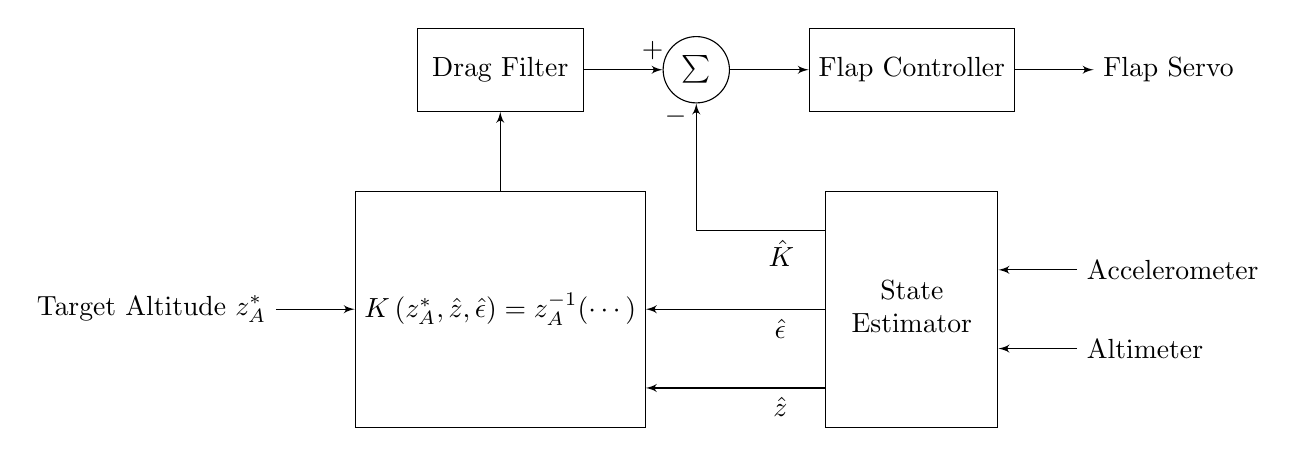
\begin{tikzpicture}[auto, >=latex']
		\node(dragconst)[block]{Drag Filter};
		\node(dragerror)[sum, right=of dragconst];
		\node(dragcontrol)[block, right=of dragerror]{Flap Controller};
		\node(flappos)[output, right=of dragcontrol]{Flap Servo};
		
		\draw[->] (dragconst) -- node[suminplus]{} (dragerror);
		\draw[->] (dragerror) -- (dragcontrol);
		\draw[->] (dragcontrol) -- (flappos);
		
		\node[block, below=of dragcontrol, minimum height=3cm](estimator){\begin{tabular}{c}State\\Estimator\end{tabular}};
		\node[input, right=of estimator, yshift=0.5cm](accel){Accelerometer};
		\node[input, right=of estimator, yshift=-0.5cm](alt){Altimeter};
		\node[block, below=of dragconst, minimum height=3cm](altcalc){$K\left(z_A^*,\hat{z},\hat{\epsilon}\right)=z_A^{-1}(\cdots)$};
		\node(apogee)[input, left=of altcalc]{Target Altitude  $z_A^*$};
		
		\draw[->] (accel) -- ([yshift=0.5cm]estimator.east);
		\draw[->] (alt) -- ([yshift=-0.5cm]estimator.east);
		\draw[->] (apogee) -- (altcalc);
		\draw[->] ([yshift=-1cm]estimator.west) -- node[near start]{$\hat{z}$} ([yshift=-1cm]altcalc.east);
		\draw[->] (estimator.west) -- node[near start]{$\hat{\epsilon}$} (altcalc.east);
		\draw[->] ([yshift=1cm]estimator.west) -| node[pos=0.17]{$\hat{K}$} node[suminminus,pos=0.95]{} (dragerror);
		\draw[->] (altcalc) -- (dragconst);
		\end{tikzpicture}
		\caption{DABS Control System Block Diagram}
		\label{fig:controlblock}
	\end{figure}

	The inversion of \eqref{eqn:kapogee} in the drag prediction step unfortunately cannot be done in closed form since $K$ is present both inside and outside the natural log.  However using the derivative in \eqref{eqn:kderiv} the root can be determined to an acceptable precision in a few iterations of Newton's method, using the update step in \eqref{eqn:newtons}.
	
	\begin{equation} \label{eqn:newtons}
		K^+ = K - \left(z_A(K) - z_A^* \right) \left(\frac{dz_A}{dK}\right)^{-1}
	\end{equation}
	
	This can be simplified further which will be useful for efficient computation.  Substituting \eqref{eqn:kderiv}:
	
	\begin{empheq}[box=\fbox]{equation}
		K^+ = K\left(1 + \dfrac{z_A - z_A^*}{\left(z_A-z_0\right) - \dfrac{\epsilon_0}{g+\epsilon_0 K}}\right) = K\left(1 + \dfrac{\Delta z - \Delta z^*}{\Delta z - \left(g/\epsilon_0+K\right)^{-1}}\right)
	\end{empheq}
	
	Where $\Delta z^* = z_A^* - z_0$ and $\Delta z = z_A - z_0 = \frac{1}{K}\ln\left(1 + \frac{K}{g}\epsilon_0\right)$ from \eqref{eqn:kapogee}.  A test script written in python shows that very good convergence ($<0.0001\si{\percent}$) can be had in just 2 iterations once a reasonable starting value is obtained (initial convergence from poor initial guess $\sim\!6$ iterations).  Because the function is not defined when the argument of the logarithm is negative, an additional check was performed to identify when a negative $K$ is predicted, and instead the $K$ is divided by 2.  This is still guaranteed to produce a closer estimate since the current $K$ must be in the negative section of the curve (past the root) in a low slope region in order to get a negative prediction (since the derivative is negative everywhere).
	
	\subsection{State Estimation}
	
	The parameters we will need to estimate are $a_d$, $v$, $z$, and $\theta$ where $a_d$ is the acceleration due to drag (this is actually measured directly since the accelerometer does not register gravity) and $\theta$ is the angle to vertical.  From this we obtain everything needed to calculate the (angle corrected) apogee prediction ($K,\epsilon,z,\theta$).  $z$ and $\theta$ are obviously is available directly from the vector, and $\epsilon$ is defined to be $v^2/2$.  $K$ is found as it is the propotionality constant between $\epsilon$ and $a_d$, which are both available ($K=a_d/\epsilon=2a_d/v^2$).
	
	We have pretty much direct measurement of $a_d$ and $z$ with the accelerometer and altimeter, respectively.  $v$ can be interpolated then, both by differentiation of $z$ (lengthened by $\sec\theta$) and by integration of the acceleration in the direction of motion ($a_d+g\cos\theta$).  $\theta$ is very difficult to estimate on its own, and will really require that we track our full spatial orientation.  Pure gyro integration would eventually become unstable, but with the addition of a magnetometer we will be able to discipline this estimate.
	
	Because of the high accuracy and data rate available from the IMU (accelerometer and gyroscope), we will not perform any additional filtering and will use the directly measured values, and will assume a constant covariance.  The altitude \textit{will} be estimated both by the exact altimeter measurement and the double integration of the accelerometer since over short timescales the integration may actually be more precise.  As such, the only values that will be estimated by the position estimator are $v$ and $z$.
	
	The angular estimate will be done entirely independent from position for simplicity (and the effect of $\theta$ covariance will not be incoporated in the position update step).  Because an attitude filter was already designed for MMD that uses both gyro and magnetometer, it can be mostly re-purposed.  As such, we will be producing an attitude quaternion --- perhaps somewhat overkill for this application but it does actually make it somewhat easier to compute the angle $\theta$.
	
	The details of both the position and angular filters are provided in the next two sections.  Where applicable, the symbol convention of the Kalman Filter Wikipedia page is used for the various model and covariance matrices.
	
	\subsubsection{Position Estimator}
	
	As mentioned in the previous section, because of the high accuracy of the accelerometer, that measurement will be taken as correct, with a constant covariance assigned based on the sensor specs.  The estimator will be a standard linear Kalman filter assuming the estimate of $\theta$ coming from the angular estimator to be exact.  The only estimated parameters will be $v$, the magnitude of the velocity, and $z$ the altitude.  Using the usual kinematic equations and noting that the angle between $\vec{v}$ and $\uvec{z}$ is $\theta$, the position update model becomes: 
	
	\begin{equation}
		\bmat{v^+\\z^+} = \bmat{1&0\\dt\cos\theta&1}\bmat{v\\z} - \bmat{dt\\\frac{1}{2}dt^2\cos\theta}a_d - \bmat{dt\cos\theta\\\frac{1}{2}dt^2}g
	\end{equation}
	
	In this equation the main source of process noise is the variance of the accelerometer measurements which we assume constant as before.  Since the acceleration affects the state through the acceleration term vector, the process noise matrix is the transformed covariance as \eqref{eqn:posqmat}.  Additional process noise (to account for other disturbances and model imperfections) can be also added on top of this base variance.
	
	\begin{equation}\label{eqn:posqmat}
		\mat{Q} = \bmat{dt\\\frac{1}{2}dt^2\cos\theta} \sigma_{accel}^2 \bmat{dt&\frac{1}{2}dt^2\cos\theta} = \bmat{dt^2&\frac{1}{2}dt^3\cos\theta\\\frac{1}{2}dt^3\cos\theta&\frac{1}{4}dt^4\cos^2\theta}\sigma_{accel}^2
	\end{equation}
	
	As for the measurement model, the only sensor that measures these values is the altimeter (since the accelerometer is being taken as truth).  Since the altitude $z$ is already a member of the state vector directly, the model is extremely simple:
	
	\begin{equation}
		\mat{H} = \bmat{0&1} \qquad R = \sigma_{alt}^2
	\end{equation}
	
	\subsubsection{Attitude Estimator} \def\aerr{\tvec{\theta}}
	
	Since this estimator is based heavily on the one designed for the MMD Tracker, only the important high level parameters for this application are defined and discussed here.  For a full explanation of the symbols, parameters and filter architecture it is recommended to review the report on that estimator which can be found in the RRS Google Drive under Club Projects/MMD Tracker/Estimator Design (\textit{ECSE 4440: Control Systems Engineering Final Project Report}; Patrick Love, 2019).
	
	The main difference between this filter and the MMD one is that we will similarly take the gyro values as correct, with gyro noise entering the model as process noise rather than measurement covariance.  Additionally, the accelerometer will not be used in any way to aid orientation, mainly since the simplified $v$, $z$ position filter does not estimate full inertial acceleration from which the measurement with the gravity vector could be predicted.
	
	The angular error deviation can be predicted exactly as the MMD design ignoring the angular acceleration term.  As before, when calculating the expectation the $\aerr$ term will always be zero as guaranteed by the reset step.  Since we only consider orientation for this filter, this is also the only element of the error vector.  So the full model update equation is:
	
	\begin{equation}
		\aerr^+ = \aerr + dt\tanc\left(\frac{\omega dt}{2}\right)\vec{\omega}
	\end{equation}
	
	The difference begins to arise in the covariance as now $\vec{\omega}$ is the source of process noise.  Nonetheless the process of remapping the gyro noise through the matrix is still straightforward, even more so since it is actually just a scalar in this case (once linearized anyway).  This means the gyro-induced process noise is:
	
	Angular Model Covariance
	\begin{equation}
		\mat{Q} = \sigma_{gyro}^2 dt^2\tanc^2\left(\frac{\omega dt}{2}\right) \mat{I_{3\times3}}
	\end{equation}
	
	As with the position model, additional process noise could be added to this to account for other model errors.
	
	For the use of the magnetometer for orientation measurement, the same normalized unit vector comparison is used.  That is the measurement $\uvec{z}$ is the normalized vector in the direction of the measured magnetic field $\vec{B}$ ($\uvec{z} = \frac{\vec{B}}{B}$).  The model equations are then the same ($\uvec{v}$ is the reference magnetic field direction):
	
	\begin{equation}
		\vec{h}(\hat{q}) = A(\hat{q})\uvec{v}\qquad\mat{H} = [A(\hat{q})\uvec{v}]_\times\qquad
		\mat{R} = \frac{\sigma_{mag}^2}{B^2}\mat{I_{3\times 3}}
	\end{equation}
	
	\paragraph{Computing $\theta$ from the Attitude Quaternion}
	
	In order to calculate the angle from vertical, the easiest way is to dot the body z axis with the inertial z-axis.  The quaternion $q$ was defined to rotate the inertial basis vectors to the body basis, so we need to dot $\uvec{z}$ with $\mat{M}(q)\uvec{z}$.  Noting that in the inertial frame $\uvec{z} = \bmat{0&0&1}^T = \delta_{i3}$:
	
	\begin{equation}
		\cos\theta = \uvec{z} \cdot \mat{M}(q)\uvec{z} = \delta_{i3} M(q)_{ij} \delta_{j3} = M(q)_{33} = 1-2\left(q_x^2+q_y^2\right)
	\end{equation} 
	
	Where the final result is the extracted component of the quaternion derived rotation matrix.  Even better, the actual value of $\theta$ is actually never used, and it is only $\cos\theta$ that appears in the position filter and in the corrected apogee estimator.  Thus it is not even necessary to perform the (somewhat expensive) $\arccos$ operation or the subsequent normal trigonometry in the other formulae.
	
	\subsection{Actuator Dynamics}
	
	
	
\end{document}
